\documentclass[10pt,a4paper]{article}
\usepackage[margin=19mm]{geometry}
\usepackage[T1]{fontenc}
\usepackage[utf8]{inputenc}
\usepackage{amsmath,amssymb,bm,booktabs,longtable,array,graphicx,xcolor}
\usepackage[hidelinks]{hyperref}
\newcommand{\vswirl}{\mathbf{v}_{\!\boldsymbol{\circlearrowleft}}}
\newcommand{\rhoF}{\rho_{\!f}}
\newcommand{\rhoE}{\rho_{\!E}}
\newcommand{\rhoM}{\rho_{\!m}}
\newcommand{\rc}{r_c}
\title{A077 -- Electron Layer \& Leapfrogging Unknots\\\large Falsification Protocol and Report -- v0.1.2}
\author{SST-Workbench -- mathematical research track}
\date{28 October 2026}
\begin{document}
\maketitle
\noindent\fcolorbox{black}{gray!8}{\parbox{0.96\linewidth}{\textbf{SCIENTIFIC STATUS: DEVELOPMENT / DIAGNOSTIC ONLY.} Numerical ring-parity and a three-dimensional finite-width periodic Euler pilot do not prove an electron, quantized orbital layers, material vortex-tube stability, or spin $1/2$. Original A077-v0.1.0 remains unmodified.}}

% SST-REPORT-SECTION:IDENTIFICATION
\section{Identification, scope, and status}
Catalog family \texttt{A077\_Electron\_Layer\_Leapfrogging}; version \texttt{A077-v0.1.2}. This release is a new, standalone instance produced by the official Framework v1.1.0 generator, with an embedded hash-verified source snapshot. Its parent is A077-v0.1.1. This release changes only the lifecycle of G10 and its associated tests and reporting; the reduced-ring and separate Euler-pilot numerical equations are preserved. This project implements a reduced circular-filament control and an optional, separate periodic Fourier--Galerkin Euler pilot. Numerical evidence is not physical validation.

% SST-REPORT-SECTION:QUESTION
\section{Falsifiable scientific question and objectives}
Do unforced, mutually induced coaxial closed ring filaments exhibit resolution-consistent overtaking events without requiring discrete energy levels? Does adding an independent azimuthal (toroidal) velocity component to a finite-width, meridional (poloidal) periodic Euler flow generate an additional, demonstrable dynamical invariant or a physically derived spinorial response? \emph{The second question remains unresolved by this first finite-width pilot.} Vertical ring-order permutations are never labeled electron levels $N\to N\pm1$.

% SST-REPORT-SECTION:HYPOTHESES
\section{Competing hypotheses and decision rules}
$H_0$: continuous classical ring coordinates, circulation-sign reversal, and smooth Euler velocity fields generate no intrinsically quantized spectrum or $2\pi$ sign-flipping spinor by themselves. $H_1$: a continuum-qualified material carrier yields independently stable, discrete intrinsic states and a non-postulated spinor-state representation whose $2\pi$ holonomy is $-1$ and whose $4\pi$ holonomy is $+1$. In v0.1.2, classical rank swaps are measured but do not test $H_1$. Absent independent physical representation, \texttt{G8 = UNRESOLVED}; a trivial $2\pi$ periodicity test of an ordinary vector field is not a spinor test.

% SST-REPORT-SECTION:ASSUMPTIONS
\section{Assumptions, applicability and excluded regimes}
The target fluid is incompressible, inviscid and unforced with universal evolution time $t$. \emph{Reduced-ring model:} ring centrelines are constrained to circles, cross-section follows an imposed $a_i^2R_i$ proxy, the mutual induction kernel is softened, and the self-speed uses a thin-core closure. No stretching, field pressure or nonaxisymmetric modes are resolved. \emph{Finite-width field pilot:} periodic cube, smooth core-scale data, Fourier--Galerkin $2/3$ de-aliasing, Leray projection and fourth-order Runge--Kutta (RK4). Vorticity is resolved on the chosen spectral grid but no topological/material core is identified and no continuum convergence is certified. Thin-core near-contact, unbounded-domain extrapolation, spinorial topology, photon emission and atmospheric plasma dynamics are outside the validated domain.

% SST-REPORT-SECTION:SYMBOLS
\section{Notation, units and dimensional consistency}
\begin{center}\small\begin{tabular}{llll}\toprule
Symbol & Quantity & SI unit & Dimension\\\midrule
$R_i,z_i,a_i$ & ring radius, axial position, core proxy & m & $L$\\
$\Gamma_i$ & signed circulation & m$^2$ s$^{-1}$ & $L^2T^{-1}$\\
$\rhoF$ & effective fluid density & kg m$^{-3}$ & $ML^{-3}$\\
$t,\,t_0$ & absolute evolution time, chosen time scale & s & $T$\\
$\mathbf u,\boldsymbol\omega$ & velocity, vorticity & m s$^{-1}$, s$^{-1}$ & $LT^{-1}$, $T^{-1}$\\
$E,H$ & kinetic energy, kinematic helicity & J, m$^4$ s$^{-2}$ & $ML^2T^{-2},L^4T^{-2}$\\
$\delta_s$ & sampled surface clearance & m & $L$\\\bottomrule\end{tabular}\end{center}
Conditional SST scaling, \emph{not a fitted electron prediction}: $R_0=\rc=1.40897017\times10^{-15}\,$m, $\lVert\vswirl\rVert=1.09384563\times10^6\,$m s$^{-1}$, $\Gamma_0=2\pi R_0\lVert\vswirl\rVert$ and $t_0=R_0^2/\Gamma_0$. The ring code runs with $R/R_0$, $z/R_0$ and $t/t_0$; the Euler pilot is separately dimensionless with length $R_0$ and an explicitly chosen reference velocity, and no universal clock conversion is assumed.

% SST-REPORT-SECTION:EQUATIONS
\section{Exact equations and derived measurements}
\paragraph{E1 -- regularized mutual induction.} For circular source $\mathbf X_j(\varphi)=(R_j\cos\varphi,R_j\sin\varphi,z_j)$,
\begin{equation}
\mathbf u_{i\gets j}=\frac{\Gamma_j}{4\pi}\int_0^{2\pi}
\frac{\mathbf X'_j(\varphi)\times(\mathbf x_i-\mathbf X_j(\varphi))}{(\lVert\mathbf x_i-\mathbf X_j(\varphi)\rVert^2+a_j^2)^{3/2}}\,d\varphi,\quad i\ne j.
\end{equation}
This defined softened kernel is a proxy, not a resolved finite-core Euler Green function. $[\Gamma X'r/r^3]=L/T$.
\paragraph{E2 -- slender-core closure and E3 -- imposed core-volume proxy.}
\begin{align}
U_i^{\rm self}&=\frac{\Gamma_i}{4\pi R_i}\left[\log\left(\frac{8R_i}{a_i}\right)-\frac14\right],\\
a_i(t)^2R_i(t)&=a_i(0)^2R_i(0),\qquad
\dot R_i=\sum_{j\ne i}u_{R,i\gets j},\quad \dot z_i=U_i^{\rm self}+\sum_{j\ne i}u_{z,i\gets j}.
\end{align}
The coefficient $1/4$ is a model convention. $[U_i]=L/T$; $[a_i^2R_i]=L^3$.
\paragraph{E4--E6 -- crossings, surface clearance and refined root times.}
\begin{align}
\Delta z(t)&=z_2(t)-z_1(t),\qquad \Delta z(t_c)=0\text{ with a sign change},\\
\delta_s(t)&=\sqrt{(R_1-R_2)^2+(z_1-z_2)^2}-(a_1+a_2),\\
\Delta z_H(s)&=(2s^3-3s^2+1)f_0+(s^3-2s^2+s)hf'_0\\
&\quad+(-2s^3+3s^2)f_1+(s^3-s^2)hf'_1,\quad s=(t-t_0)/h.
\end{align}
The crossing estimator solves $\Delta z_H(s)=0$ only for sign-changing sampled brackets. This cubic interpolation is not exact RK4 dense output; root times require independent time-step convergence. An observed positive $\delta_s$ is a sampled circular-tube clearance proxy, not a guarantee of continuum core disjointness.
\paragraph{E7--E9 -- finite-width periodic Euler pilot.}
\begin{align}
\partial_t\mathbf u&=\mathcal P_{\mathcal K}(\mathbf u\times\boldsymbol\omega),\quad
\boldsymbol\omega=\nabla\times\mathbf u,\quad\nabla\cdot\mathbf u=0,\\
\mathbf u(0)&=\mathcal P_{\mathcal K}\left[\nabla\times(A_{\varphi}\mathbf e_{\varphi})+v_{\varphi}\mathbf e_{\varphi}\right],\\
E&=\frac{\rhoF}{2}\int |\mathbf u|^2\,d^3x,\qquad
H=\int\mathbf u\cdot\boldsymbol\omega\,d^3x.
\end{align}
The smooth Gaussian toroidal seed has independently specified meridional and azimuthal velocity amplitudes; $v_\varphi$ is not a new circulation quantum. $\mathcal P_{\mathcal K}$ is the divergence-free Fourier projection with spectral cutoff. Dimensions are $[\partial_t\mathbf u]=[\mathbf u\times\boldsymbol\omega]=LT^{-2}$, $[E]=ML^2T^{-2}$, $[H]=L^4T^{-2}$. The spectral pilot uses normalized coordinates and diagnostics. Its discretized dynamics do not establish the continuum vorticity-knot topology.
\paragraph{Automatic equation register.}
\IfFileExists{AUTO_SCIENCE_CONTRACT.tex}{% AUTO-GENERATED. Do not edit; generated from frozen science_contract.json.
\subsection*{Machine-readable science contract}
\begin{description}
\item[Research question] Do regularized coaxial vortex-ring rank swaps and smooth independent meridional/azimuthal finite-width Euler initial fields yield convergent dynamics; is a new nonimposed spinorial two-turn response demonstrated?
\item[Objective] Separate classical geometric ring overtakings and numerical backend parity from true discrete energy levels, finite-core Euler carrier dynamics, and genuine spin-1/2 representation. v0.1.2 adds dense trace, Hermite root/event convergence, clearance, a periodic 3D Euler research pilot and independent numerical G5/G10 gates. v0.1.2 repairs G10 evaluation order only; no numerical physics kernel, target or threshold is modified.
\item[$H_0$] Continuous classical ring-overlap-free trajectories, sign-dependent velocity and smooth Galerkin Euler evolution do not in themselves produce quantized intrinsic energies, electron identity, or projective spinor holonomy.
\item[$H_1$] An independently certified continuum finite-core Euler model exhibits discrete, parameter-robust intrinsic eigenclasses and uniquely derived spinorial 2pi/4pi holonomy without imposed state phase. This hypothesis is NOT evaluated in v0.1.2.
\end{description}
\subsubsection*{Registered equations}
\paragraph{E1: regularized pairwise ring induction quadrature}
\begin{equation}
u_{i<-j}=Gamma_j/(4pi) integral_0^{2pi} [X_j^prime(phi) cross (x_i-X_j(phi))]/(|x_i-X_j(phi)|^2+a_j^2)^(3/2) dphi
\end{equation}
\noindent\textit{Dimensional check:} (L\textasciicircum{}2/T)*L*L/L\textasciicircum{}3=L/T\\
\paragraph{E2: slender-core self speed, explicit model choice}
\begin{equation}
U_i=Gamma_i/(4pi R_i)[ln(8R_i/a_i)-1/4]
\end{equation}
\noindent\textit{Dimensional check:} (L\textasciicircum{}2/T)/L = L/T\\
\paragraph{E3: imposed thin-tube area-length proxy}
\begin{equation}
a_i^2(t)R_i(t)=a_i^2(0)R_i(0)
\end{equation}
\noindent\textit{Dimensional check:} L\textasciicircum{}3=L\textasciicircum{}3\\
\paragraph{E4: axial-order crossing event}
\begin{equation}
Delta z(t)=z_2(t)-z_1(t); Delta z(t_cross)=0 with sign reversal
\end{equation}
\noindent\textit{Dimensional check:} Delta z has L, t\_cross has T\\
\paragraph{E5: coaxial minimal core tube clearance}
\begin{equation}
d_surf=sqrt((R_1-R_2)^2+(z_1-z_2)^2)-(a_1+a_2)
\end{equation}
\noindent\textit{Dimensional check:} L-L=L\\
\paragraph{E6: cubic Hermite bracketed event estimator}
\begin{equation}
Delta z_h(s)=(2s^3-3s^2+1)f_0+(s^3-2s^2+s)h f_0prime+(-2s^3+3s^2)f_1+(s^3-s^2)h f_1prime
\end{equation}
\noindent\textit{Dimensional check:} f has L, h*fprime has L; s dimensionless\\
\paragraph{E7: periodic incompressible Euler Galerkin ODE}
\begin{equation}
partial_t u=P_K(u cross omega), omega=curl u, div u=0
\end{equation}
\noindent\textit{Dimensional check:} [u omega]=L/T\textasciicircum{}2=[du/dt]\\
\paragraph{E8: independent initial meridional and azimuthal velocity components}
\begin{equation}
u_0=P_K(curl(A_phi e_phi)+v_phi e_phi), with v_phi=b*sum(r/R_i)*Gaussian_i
\end{equation}
\noindent\textit{Dimensional check:} [curl A]=L/T; [v\_phi]=L/T, b dimensionless if velocity normalized\\
\paragraph{E9: Euler helicity and kinetic energy diagnostics}
\begin{equation}
E=(rho_f/2) integral |u|^2 dV; H=int u dot curl u dV
\end{equation}
\noindent\textit{Dimensional check:} [E]=ML\textasciicircum{}2/T\textasciicircum{}2; [H]=L\textasciicircum{}4/T\textasciicircum{}2\\
\subsubsection*{Registered code-to-mathematics steps}
\begin{enumerate}
\item \textbf{S1} [G1; equations E1]: Validate frozen framework and source input exact SHA-256; load analytic ring scenarios
\item \textbf{S2} [G2; equations E1, E2, E3]: Run full 401-sample reduced-ring RK4 trajectory and write raw CSV with conditional SI conversion
\item \textbf{S3} [G2; equations E4, E5, E6]: Locate bracketed cubic Hermite root crossings and minimum sampled tube clearance
\item \textbf{S4} [G2; equations E4, E6]: Independent ntheta and dt refinements at same fixed t\_final; match event counts and root shifts
\item \textbf{S5} [G5; equations E1, E2]: Execute pybind11 science kernel and numeric reference in same instance; pass only if actual execution and parity
\item \textbf{S6} [G10; equations E1, E2]: After backend matrix framework assesses two genuinely executed backend categories and independent numeric parity G10 is deliberately left unrecorded during the science pipeline and assessed by the original framework runner after AUTO\_BACKEND\_MATRIX.json exists; lack of second backend is UNRESOLVED, non-parity FAIL, accepted parity PASS (numeric only).
\item \textbf{S7} [G8; equations E7, E8, E9]: Run optional 3D Fourier Galerkin Euler research pilot, separate no-toroidal and + and - azimuthal swirl amplitudes
\item \textbf{S8} [G8; equations E7]: Do not score spinor without physically identified state representation, holonomy and held-out continuum convergence
\end{enumerate}
}{The equation-to-code register is generated from the frozen science contract.}

% SST-REPORT-SECTION:ALGORITHM
\section{Equation-to-code sequence and source mapping}
\begin{enumerate}
\item Load and hash \texttt{configs/pilot.json} and its four disclosed analytic sign controls.
\item Evaluate E1--E3 using \texttt{science/ring\_model.py}, write complete time series with all 401 samples of each case and conditional SI conversion.
\item Compute E4--E6 in \texttt{science/diagnostics.py}: bracketed cubic Hermite event roots, minimum centreline/core clearance, and three-level angular and temporal refinements at identical final time.
\item Independently execute native C++ via \texttt{native/cpp/native.cpp} and compare with Python, recording compiled module hash, source hash and common input hash. The Framework rechecks execution and numeric parity under G10. The science pipeline deliberately leaves G10 unrecorded; the unchanged Framework runner computes and records G10 \emph{after} the actual multi-backend matrix is written. An early UNRESOLVED placeholder would suppress this official G10 evaluation.
\item Optionally, separately run \texttt{python -m science.euler\_field} using \texttt{configs/euler\_pilot.json}, generating three finite-width velocity-field cases: azimuthal amplitude $0$, $+b$, and $-b$.
\item Record Euler energy, helicity, enstrophy, divergence, step size and spectral-grid configuration. Require future independent full spatial/temporal/core-width studies before any physical stability claim.
\item Preserve G3, G4 and G8 as unresolved. Any future reveal is a distinct private, preregistered operation, never part of diagnostics.
\end{enumerate}

% SST-REPORT-SECTION:SOURCES
\section{Provenance, sources and independence}
The four ring controls are deterministic analytic input conditions, not four independent laboratory datasets. The ring quadrature and timestep levels are numerical refinements, not independent source families. The Euler Galerkin module is an independent \emph{model class} from the reduced filament, not an independently validated material vortex-tube solver. No E010 knot atlas is copied into this instance, no physical electron mass/charge targets are used to fit the kernels, and no private reveal data enter public blind archives. The self-contained Framework v1.1.0 runtime source is pinned with its exact 142-file SHA-256 inventory; the frozen protocol has its own byte-exact manifest and commitments.

% SST-REPORT-SECTION:GATES
\section{Gate dependency graph and scientific ceilings}
\small\begin{longtable}{p{.12\linewidth}p{.62\linewidth}p{.18\linewidth}}\toprule Gate & Test and qualifying evidence & Max authority now\\\midrule\endhead
G0 & Official frozen protocol and embedded source snapshot & TECHNICAL\\
G1 & Analytic source/control hashes & TECHNICAL\\
G2 & Angle/time refinement, Hermite events, checks; no continuum Euler & PROXY-ONLY\\
G3 & Blind, held-out intrinsic spectral quantization & UNRESOLVED\\
G4 & Independent full-field finite-core continuum confirmation & UNRESOLVED\\
G5 & Executed native pybind11 ring kernel parity, independent of G4 & NUMERIC-ONLY\\
G6 & GPU science kernel, only if actually executed & NOT APPLICABLE\\
G7 & External source-family replication & NOT APPLICABLE\\
G8 & Euler continuum, intrinsic layers and spinorial bundle & UNRESOLVED\\
G9 & Commitment-verified private reveal after qualified gates & DEFERRED\\
G10 & Post-backend Framework two-of-three executed backends plus preregistered numerical parity; no early pipeline placeholder & NUMERIC-ONLY\\\bottomrule\end{longtable}\normalsize
G5 and G10 require only G2: actual numerical parity must not be causally blocked by unrelated physical G4. G10 is intentionally left unrecorded by the A077 science pipeline before the official backend matrix: the framework runner then evaluates it from verified scientific execution evidence and the preregistered tolerance. Valid Python/C++ parity may qualify G10; a missing second backend must return UNRESOLVED and divergent numeric output must return FAIL. No fallback, manufactured evidence or premature PASS is permitted. G8 continues to depend on genuinely independent physical G3/G4/G7. A G10 PASS is not a physical G8 PASS; the framework separates observed status from evidence qualification. The additional physical subtests P01--P07 are described by raw diagnostics and research limitations, not promoted to substitute framework gates.

% SST-REPORT-SECTION:NUMERICS
\section{Numerical refinements and predeclared thresholds}
For $t_f/t_0=5$ and reference same-sign pair $R=(1,0.8)$, $z=(-.15,+.15)$, $\Gamma=(+1,+1)$ and initial $a/R=.1$:
\begin{itemize}
\item Angular quadrature levels $n_\varphi=(48,96,192)$ at 400 RK4 steps.
\item Temporal levels $(200,400,800)$ steps at $n_\varphi=96$.
\item Relative end-state tolerances $2\times10^{-2}$ (angular), $10^{-2}$ (temporal); both crossing counts must agree and maximum paired root shift $\leq 2\times10^{-3}$ in $t/t_0$.
\item Sampled clearance $\delta_s>0$ is a separate domain check; its failure blocks a non-contact physical interpretation, even if the proxy numerical gate passes.
\item Euler pilot uses $(n,L,t_f,\Delta t)=(24,8,.02,.002)$ and only illustrates short-time bounded Galerkin evolution; no spatial, temporal or core convergence is certified. A future physical gate requires $n$-refinement and $\Delta t$-refinement at fixed physical end time, \emph{plus} width, box and nonaxisymmetric perturbation studies.
\end{itemize}
Small endpoint differences and exact machine-level conservation can result from the Fourier--Galerkin truncation; neither establishes a physical restoring force, self-confinement or stable particle state.

% SST-REPORT-SECTION:BACKENDS
\section{Backend authority, cross-checks and Windows build}
The Python NumPy binary64 code is the numerical reference. The independent native C++17 pybind11 ring kernel is accepted only after a genuine compile/execution, signed compiled binary/source hashes and $\ell_2$ parity $\leq10^{-10}$. Framework G10 further requires at least two real scientific categories from Python/C++/GPU. Intel Arc XPU and NVIDIA CUDA are a single GPU category, not two. Hardware preflight is not scientific execution. A missing C++/GPU implementation keeps FULL/CERTIFY unqualified; no silent Python fallback. DD32/FP32x2 remains \texttt{SCREENING\_ONLY}. The optional periodic Euler pilot is currently Python-only, so native ring parity does not certify the independent field solver.

% SST-REPORT-SECTION:BLINDNESS
\section{Blinding, private keys, and reveal isolation}
The protocol contains no target-tuned electron mass, electric charge, Planck constant, measured spin projection, or discovered energy-level labels. The Framework creates new private opaque-ID and reveal-nonce bytes for this \emph{new} version; they are stored under \texttt{private/}, never in a BLIND ZIP. The blind manifest, ledger, and source hashes are immutable once frozen. Reveal is blocked unless the independent scientific gate and commitment policy qualify it. Repeated BASIC/FULL/CERTIFY runs have unique identities and retain older outputs. The distributed source archive is private because it contains generated private credentials.

% SST-REPORT-SECTION:STATISTICS
\section{Null model, multiplicity and interpretation controls}
The deterministic reduced-model trajectories have \emph{no stochastic null ensemble}. Counting RK4 timesteps, sign configurations or grid levels as independent replicates is prohibited. The trial is not a statistical discovery of quantum levels; no $p$-values or multiple-testing claims are made. Future discrete-mode studies require blinded held-out parameters, a preregistered operator and continuum/finite-core null, familywise correction if multiple candidate modes are searched, and independent source confirmation.

% SST-REPORT-SECTION:RESULTS
\section{Measured results and automatic immutable run provenance}
\IfFileExists{AUTO_RESULTS.tex}{% AUTO-GENERATED. Do not edit.
\subsection*{Automatic run provenance}
\begin{longtable}{p{0.28\linewidth}p{0.64\linewidth}}
\toprule
Field & Recorded value \\
\midrule
Run ID & 20261030T124229778258Z-\allowbreak{}240446e4 \\
Run phase & BLIND \\
2-of-3 backend execution & EXECUTION\_\allowbreak{}CONTRACT\_\allowbreak{}PASS \\
Executed backend categories & py, cpp \\
GPU provider & intel \\
Protocol bundle SHA-256 (byte exact) & de17289fba74\allowbreak{}471bfa087a95\allowbreak{}91a6997b48b2\allowbreak{}acf287b9bf01\allowbreak{}15f12c12b7ca\allowbreak{}7f47 \\
Portable protocol diagnostic SHA-256 & bee9f8bfa773\allowbreak{}dfc6038d0c40\allowbreak{}bbfa5205793b\allowbreak{}f7005779bc92\allowbreak{}05d5f35009e5\allowbreak{}079e \\
Framework schema & SST-\allowbreak{}FALSIFIER-\allowbreak{}PROTOCOL-\allowbreak{}2 \\
Python & 3.13.9 (tags/\allowbreak{}v3.13.9:8183fa5, Oct 14 2025, 14:09:13) [MSC v.1944 64 bit (AMD64)] \\
Platform & Windows-\allowbreak{}11-\allowbreak{}10.0.26300-\allowbreak{}SP0 \\
Science evidence SHA-256 & a4c0c24ccdf4\allowbreak{}1463590fb1e2\allowbreak{}d17377af98f5\allowbreak{}65bae653efc8\allowbreak{}b0107de8138f\allowbreak{}0a7a \\
Final output manifest & See OUTPUT\_\allowbreak{}MANIFEST.json (finalized after PDF and report metadata) \\
\bottomrule
\end{longtable}
\subsubsection*{Gate ledger}
\begingroup\small\setlength{\tabcolsep}{3pt}\begin{longtable}{p{0.07\linewidth}p{0.19\linewidth}p{0.31\linewidth}p{0.29\linewidth}}
\toprule
Gate & Status & Question & Reason \\
\midrule
{\ttfamily\scriptsize G0} & {\ttfamily\footnotesize PASS} & Official frozen v1.1.0 runtime integrity? & Framework frozen protocol and embedded runtime verified before science. \\
{\ttfamily\scriptsize G1} & {\ttfamily\footnotesize PASS} & Analytic source/\allowbreak{}initial data provenance? & Frozen analytic case definitions and source hashes; not independent empirical observations. \\
{\ttfamily\scriptsize G2} & {\ttfamily\footnotesize PASS} & Reduced-\allowbreak{}model numerical and dimensional controls? & Separate angle-\allowbreak{}quadrature and ODE time-\allowbreak{}step convergence with event-\allowbreak{}root tests; no 3D Euler authority. \\
{\ttfamily\scriptsize G3} & {\ttfamily\footnotesize UNRESOLVED} & Target-\allowbreak{}free spectral discreteness rather than rank swaps? & No held-\allowbreak{}out eigenvalue spectrum or discrete level detection, geometric rank swaps are classical. \\
{\ttfamily\scriptsize G4} & {\ttfamily\footnotesize UNRESOLVED} & Independent full Euler field/\allowbreak{}held-\allowbreak{}out source confirmation? & No independent finite-\allowbreak{}core continuum Euler confirmation with space/\allowbreak{}time/\allowbreak{}core convergence. \\
{\ttfamily\scriptsize G5} & {\ttfamily\footnotesize PASS} & Does the actually executed independent C++ pybind kernel numerically agree with Python within the preregistered tolerance? & Actually executed instance pybind11 C++ ring science kernel; numeric parity only. \\
{\ttfamily\scriptsize G6} & {\ttfamily\footnotesize NOT\_\allowbreak{}APPLICABLE} & Optional genuine GPU numerical screening (no GPU means NOT\_\allowbreak{}APPLICABLE)? & Disabled by framework profile \\
{\ttfamily\scriptsize G7} & {\ttfamily\footnotesize NOT\_\allowbreak{}APPLICABLE} & Independent source-\allowbreak{}family replication, not refinement/\allowbreak{}repeated run? & Disabled by framework profile \\
{\ttfamily\scriptsize G8} & {\ttfamily\footnotesize UNRESOLVED} & Do continuum full-\allowbreak{}Euler and spinorial mechanism gates close independently? & Independent toroidal/\allowbreak{}poloidal finite-\allowbreak{}width Euler pilot exists but is not continuum-\allowbreak{}certified; no spinor/\allowbreak{}field topology proof or experimental electron evidence. \\
{\ttfamily\scriptsize G10} & {\ttfamily\footnotesize PASS} & After verified multi-\allowbreak{}backend execution, does Framework 1.1.0 numeric G10 qualify Python plus an independent science backend with preregistered parity? & Preregistered 2-\allowbreak{}of-\allowbreak{}3 execution and numerical tolerances satisfied; physics not certified \\
{\ttfamily\scriptsize G9} & {\ttfamily\footnotesize DEFERRED} & Only after physical gates qualify, is private reveal allowed? & Reveal is a separate, commitment-\allowbreak{}verified phase and is not executed during blind runs. \\
\bottomrule
\end{longtable}\endgroup
\subsubsection*{Scientific qualification (separate from measured gate outcomes)}
\begingroup\small\setlength{\tabcolsep}{3pt}\begin{longtable}{p{0.13\linewidth}p{0.37\linewidth}p{0.38\linewidth}}
\toprule
Gate & Evidence qualification & Blocking prerequisites \\
\midrule
G0 & QUALIFIED & none \\
G1 & QUALIFIED & none \\
G2 & QUALIFIED & none \\
G3 & UNRESOLVED & none \\
G4 & DIAGNOSTIC\_\allowbreak{}ONLY & G3 \\
G5 & QUALIFIED & none \\
G6 & NOT\_\allowbreak{}APPLICABLE & none \\
G7 & NOT\_\allowbreak{}APPLICABLE & G4 \\
G8 & DIAGNOSTIC\_\allowbreak{}ONLY & G3, G4, G7 \\
G10 & QUALIFIED & none \\
G9 & DEFERRED & G8 \\
\bottomrule
\end{longtable}\endgroup
\subsubsection*{Numeric backend comparisons (not physical validation)}
\begingroup\small\begin{longtable}{p{0.22\linewidth}p{0.25\linewidth}p{0.42\linewidth}}
\toprule
Backend & Relative L2 error & Result/status \\
\midrule
cpp & 5.923075954129776e-16 & MEASURED\_ONLY \\
\bottomrule
\end{longtable}\endgroup
\subsubsection*{Backend manifest}
\begingroup\footnotesize\begin{verbatim}
{
  "backend_2of3": {
    "artifact": "AUTO_BACKEND_MATRIX.json",
    "counted": 2,
    "executed": [
      "py",
      "cpp"
    ],
    "status": "EXECUTION_CONTRACT_PASS"
  },
  "model": "AXISYMMETRIC_REGULARIZED_FILAMENT_PROXY",
  "note": "G5 local pybind check independent of G4; G10 deliberately not 
recorded during pipeline. Official Framework runner alone computes G10 after 
real backend matrix. No physical spin/level pass.",
  "schema": "SST-BACKEND-MANIFEST-2",
  "science_diagnostics": "science_diagnostics/scientific_diagnostics.json",
  "scientific_authority": "DEVELOPMENT_DIAGNOSTIC_ONLY"
}
\end{verbatim}\endgroup
\subsubsection*{Source manifest}
\begingroup\footnotesize\begin{verbatim}
{
  "manifest_sha256": 
"bee7a88039d6c7375b5ec2d8eb062c1766a9113ff51c2a15c5290d27e4d8841d",
  "schema": "SST-SOURCE-MANIFEST-2",
  "sources": [],
  "workbench_root": "C:\\workspace\\projects\\SST-Workbench"
}
\end{verbatim}\endgroup
}{Automatic results will be inserted from the Framework execution without changing this preregistered scientific report.}
\IfFileExists{ring_traces.pdf}{\begin{center}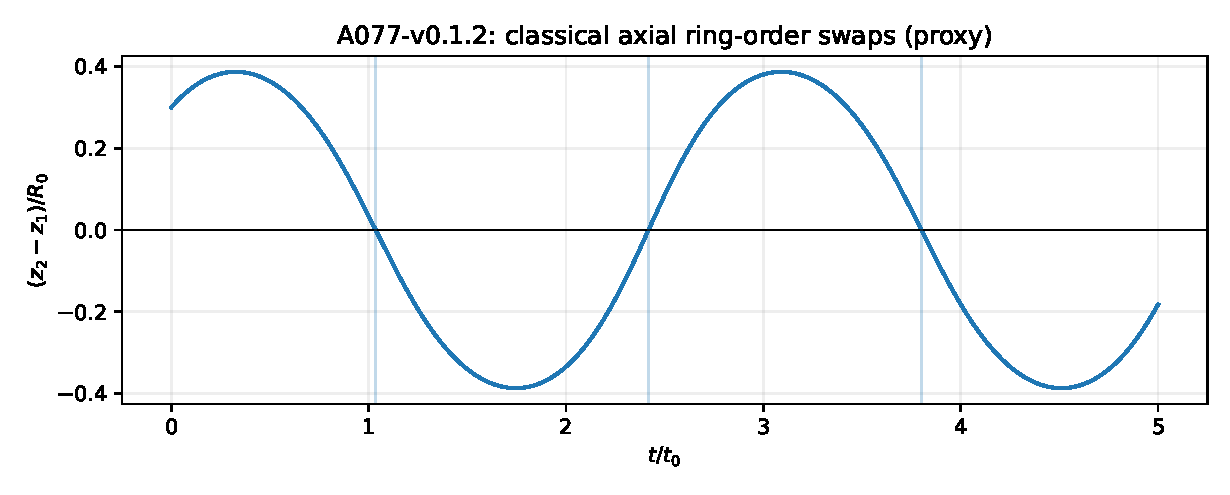
\includegraphics[width=.92\linewidth]{ring_traces.pdf}\end{center}}{}

% SST-REPORT-SECTION:INTERPRETATION
\section{Scientific interpretation, falsifiers and minimal experiments}
\textbf{ORTHODOX:} Euler circulation transport and Biot--Savart velocity reconstruction are classical conditional results. \textbf{DERIVED UNDER ASSUMPTIONS:} ring trajectory roots, clearance proxies and spectral Euler short-time diagnostics are numerical statements within their explicitly discretized models. \textbf{SPECULATIVE--RESEARCH--TRACK:} identification of CW/CCW, ring order, independent toroidal/meridional velocity, jet/sprite morphology or leapfrogging phases with electron spin-$1/2$ or physical quantum layers. A real velocity vector field is single-valued under a $2\pi$ spatial rotation; that does \emph{not} supply $\Psi(2\pi)=-\Psi(0)$ for a derived physical state, nor the exchange sign of two identical fermions. Future minimal tests: (i) fixed-time spatial/time/core refinement for the field pilot, (ii) helicity and link invariants on genuine disjoint material tubes, (iii) independent survival/repetition of internal modes, (iv) configuration-space rotation and braid loop analysis without assuming a spinorial bundle. No sprite/giant-jet ionization or electromagnetic emission is modeled.

% SST-REPORT-SECTION:REPRODUCIBILITY
\section{Exact execution, outputs and stop criteria}
\begin{verbatim}
cd /d <EXTRACTED_A077-v0.1.2>
python -m pytest -q tests
run_all.cmd BACKEND_PREFLIGHT
run_all.cmd FREEZE
run_all.cmd BASIC
run_all.cmd FULL
run_all.cmd CERTIFY
python -m science.euler_field ^
  --config configs/euler_pilot.json ^
  --output A077_euler_pilot_v0.1.2-outputs
\end{verbatim}
In \texttt{A077-v0.1.2} the Framework writes \texttt{electron\_layer\_leapfrogging\_v0.1.2-outputs/}, preserving earlier runs and publishing an immutable run-specific BLIND ZIP and its SHA-256 sidecar in the parent. Source archive must be extracted into \emph{new} version directory only. Halt physical certification on failed source hashes, absent native science backend, Euler-grid/core nonconvergence, missing evidence, frozen protocol mutation, core contact, or missing spinorial state definition. No user hardware result is claimed in advance.

\section{References}
\begin{thebibliography}{9}
\bibitem{Helmholtz1858} H. Helmholtz (1858), ``On Integrals of the Hydrodynamical Equations Which Express Vortex Motion,'' \emph{Journal f\"ur die reine und angewandte Mathematik} 55, 25--55. DOI: \url{https://doi.org/10.1515/crll.1858.55.25}.
\bibitem{Saffman1992} P. G. Saffman (1992), \emph{Vortex Dynamics}, Cambridge University Press. DOI: \url{https://doi.org/10.1017/CBO9780511624063}.
\bibitem{Davila2024} J. D\'avila, M. del Pino, M. Musso, J. Wei (2024), ``Leapfrogging vortex rings for the three-dimensional incompressible Euler equations,'' \emph{Communications on Pure and Applied Mathematics} 77, 3843--3957. DOI: \url{https://doi.org/10.1002/cpa.22199}.
\bibitem{Niemi2005} A. J. Niemi (2005), ``Exotic Statistics of Leapfrogging Vortex Rings,'' \emph{Physical Review Letters} 94, 124502. DOI: \url{https://doi.org/10.1103/PhysRevLett.94.124502}.
\bibitem{FinkelsteinRubinstein1968} D. Finkelstein and J. Rubinstein (1968), ``Connection between Spin, Statistics, and Kinks,'' \emph{Journal of Mathematical Physics} 9, 1762--1779. DOI: \url{https://doi.org/10.1063/1.1664510}.
\bibitem{Orszag1971} S. A. Orszag (1971), ``On the elimination of aliasing in finite-difference schemes by filtering high-wavenumber components,'' \emph{Journal of the Atmospheric Sciences} 28, 1074. DOI: \url{https://doi.org/10.1175/1520-0469(1971)028<1074:OTEOAI>2.0.CO;2}.
\bibitem{Dekker1971} T. J. Dekker (1971), ``A Floating-Point Technique for Extending the Available Precision,'' \emph{Numerische Mathematik} 18, 224--242. DOI: \url{https://doi.org/10.1007/BF01397083}.
\end{thebibliography}
\end{document}
